\documentclass[letterpaper,12pt,fleqn]{article}
\usepackage{matharticle}
\usepackage{mathtools}
\pagestyle{plain}
\begin{document}

\begin{center}
\Large Math-1005a Homework \#4
\end{center}

\vspace{0.5in}

\underline{Problems}

\begin{enumerate}
\item When we add two rational numbers that already have a common denominator
  then we are simply counting the number of fractional units:
  \[\frac{a}{c}+\frac{b}{c}=\frac{a+b}{c}\]
  What is the rational number equation that is suggested by the following
  diagram? Your answers should be in the form of (improper) fractions and not
  mixed numbers. You do not need to reduce your answers:

  \bigskip

  \begin{figure}[h]
    \centering
    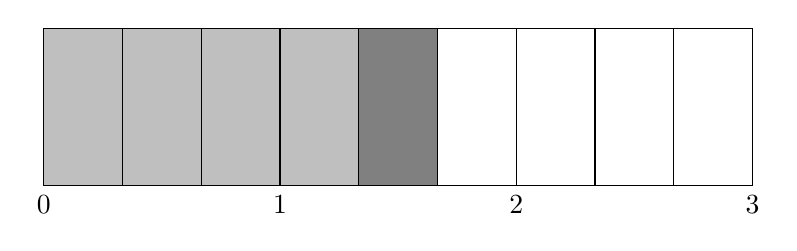
\begin{tikzpicture}
      \draw [fill=lightgray] (0,0) rectangle (1,2);
      \draw [fill=lightgray] (1,0) rectangle (2,2);
      \draw [fill=lightgray] (2,0) rectangle (3,2);
      \draw [fill=lightgray] (3,0) rectangle (4,2);
      \draw [fill=gray] (4,0) rectangle (5,2);
      \draw (5,0) rectangle (6,2);
      \draw (6,0) rectangle (7,2);
      \draw (7,0) rectangle (8,2);
      \draw (8,0) rectangle (9,2);
      \node [below] at (0,0) {$0$};
      \node [below] at (3,0) {$1$};
      \node [below] at (6,0) {$2$};
      \node [below] at (9,0) {$3$};
    \end{tikzpicture}
  \end{figure}

\item When adding and subtracting rational numbers (and fractions in general)
  that have different denominators we need to find a common denominator. One
  can always use the formula:
  \[\frac{a}{b}\pm\frac{c}{d}=\frac{ad\pm bc}{bd}\]
  but this can result in unnecessarily large values when adding and subtracting
  rational numbers. A better way is to use the least common multiple (LCM) of
  the denominators.

  Evaluate the following expressions. Your answers should be reduced (improper)
  fractions or whole numbers - not mixed numbers:
  \begin{enumerate}
  \item $\frac{7}{13}+\frac{11}{2}$
  \item $\frac{13}{14}-\frac{1}{21}$
  \item $\frac{1}{2}+\frac{3}{4}$
  \item $\frac{5}{121}-\frac{5}{22}$
  \item $10+\frac{2}{3}$
  \end{enumerate}

\item When adding and subtracting mixed numbers, we have two options. The
  first is to convert to improper fractions first. Alternatively, remember that
  mixed number notation is a shorthand for the results of the division
  algorithm:
  \[n\frac{p}{q}=n+\frac{p}{q}\]
  Thus, unlike multiplication, it is possible to add/subtract the two parts
  separately and then adjust so that the fractional part is proper. For
  example:
  \[1\frac{1}{2}+2\frac{3}{4}=1+2+\frac{1}{2}+\frac{3}{4}=3\frac{5}{4}=
  4\frac{1}{4}\]
  Be careful when subtraction is involved - the negative sign applies to both
  the whole part and the fractional part: 
  \[-1\frac{1}{2}=-1-\frac{1}{2}\]
  For example:
  \[1\frac{3}{4}-2\frac{1}{2}=1-2+\frac{3}{4}-\frac{1}{2}=-1+\frac{1}{4}=
  -\frac{3}{4}\]
  Evaluate the following expressions. Your answers should be reduced (improper)
  fractions, whole numbers, or mixed numbers:
  \begin{enumerate}
  \item $4\frac{1}{2}+5\frac{1}{3}$
  \item $16\frac{7}{15}-7\frac{2}{5}$
  \item $3\frac{1}{5}+1\frac{2}{3}$
  \item $17\frac{3}{4}-16\frac{5}{6}$
  \item $7\frac{4}{9}+3$
  \end{enumerate}

\item Sometimes it is easy to tell when one rational number is less than,
  greater than, or equal to another rational number. When the two numbers have
  the same denominator then you only need to compare the numerators. For
  example:
  \[\frac{1}{4}<\frac{3}{4}\]
  Sometimes the relative magnitude of the two numbers is obvious:
  \[\frac{100}{9}>\frac{2}{3}\]
  A fraction increases with its numerator and decreases with its denominator.
  Thus:
  \[\frac{1}{3}<\frac{2}{3}\ \mbox{and}\ \frac{1}{3}>\frac{1}{4}\]
  Furthermore, negative numbers are always less that positive numbers:
  \[-\frac{3}{4}<\frac{1}{4}\]
  In all other cases, we need to find a common denominator and then compare the
  numerators.

  For each of the following, indicate whether the first number is less than,
  equal to, or greater than the second number:
  \begin{enumerate}
  \item $\frac{8}{3}\,\framebox(20,20){}\,\frac{11}{3}$
  \item $\frac{16}{5}\,\framebox(20,20){}\,\frac{48}{15}$
  \item $\frac{4}{15}\,\framebox(20,20){}\,-\frac{4}{15}$
  \item $\frac{2}{3}\,\framebox(20,20){}\,\frac{5}{6}$
  \item $-\frac{2}{3}\,\framebox(20,20){}\,-\frac{5}{6}$
  \end{enumerate}

\item When adding and subtracting three or more rational numbers (and
  fractions in general), we need to find the least common denominator for all
  of the denominators. For example:
  \[\frac{1}{2}+\frac{2}{3}-\frac{1}{4}=\frac{6}{12}+\frac{8}{12}-\frac{3}{12}=
  \frac{11}{12}\]
  Evaluate the following expressions. Your answers should be reduced (improper)
  fractions or whole numbers - not mixed numbers:
  \begin{enumerate}
  \item $\frac{2}{3}+\frac{4}{3}+\frac{5}{3}$
  \item $\frac{11}{5}+\frac{7}{5}-\frac{6}{5}$
  \item $\frac{1}{8}-\frac{3}{4}-\frac{1}{3}$
  \item $\frac{15}{7}-\frac{3}{4}+\frac{5}{2}$
  \item $\frac{1}{3}+\frac{5}{2}+\frac{7}{5}$
  \end{enumerate}

\item Adrian and Stacey try to see who can run the farthest without stopping.
  Adrian is able to run $3\frac{1}{3}$ miles and Stacey is able to run
  $1\frac{5}{6}$ miles.
  \begin{enumerate}
  \item What is there combined mileage?
  \item How much farther did Adrian run that Stacey?
  \end{enumerate}
  Your answers can be reduced (improper) fractions, whole numbers, or mixed
  numbers.

\item After such a good workout, Adrian and Stacey go to the state fair. The
  fair is running a special: buy a souvenir bag for unlimited refills of
  popcorn. The friends decide to buy one and share it. At the end of the day,
  they realize that together they have eaten $8$ bags of popcorn. Adrian
  estimates that she alone at $5\frac{1}{4}$ bags.
  \begin{enumerate}
  \item How much popcorn did Stacey eat?
  \item How much more popcorn did Adrian eat than Stacey?
  \end{enumerate}
  Your answers can be reduced (improper) fractions, whole numbers, or mixed
  numbers.

\item Jorge, Roberto, and Jose decide to eat lunch at Mountain Mikes
  all-you-can-eat pizza buffet. Jorge eats $6$ slices, Roberto eats $8$ slices,
  and Jose eats $9$ slices. A large pizza normally has $12$ slices. How many
  large pizzas did the three friends eat?

  Your answer can be a reduced (improper) fraction, whole number, or mixed
  number.

\item Elizabeth owns a graphics design business with two employees: Jack and
  Joe. The company has just completed and been paid for a logo design project
  for a major Silicon Valley company. Elizabeth keeps half of the money for
  herself and the company. Of the remaining half, she gives $\frac{4}{5}$ to
  Jack. How much did Jack and Joe receive of the total?

  Remember to use multiplication to find the fraction of a fraction. Your
  answers should be reduced fractions.

\item The flag of Westeros (shown below) is divided into three stripes:

  \bigskip

  \begin{figure}[h]
    \centering
    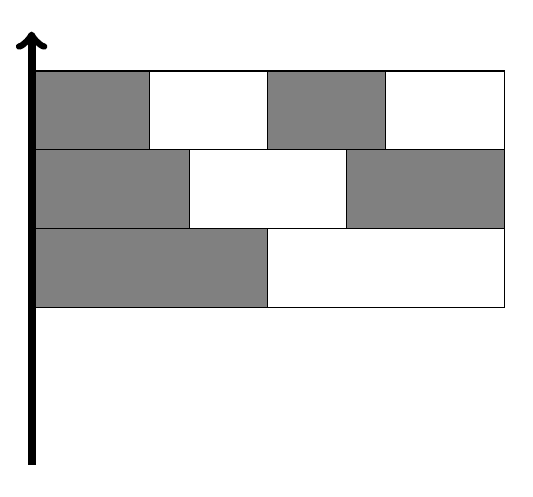
\begin{tikzpicture}[xscale=0.5]
      \draw [fill=gray] (0,0) rectangle (6,1);
      \draw (6,0) rectangle (12,1);
      \draw [fill=gray] (0,1) rectangle (4,2);
      \draw (4,1) rectangle (8,2);
      \draw [fill=gray] (8,1) rectangle (12,2);
      \draw [fill=gray] (0,2) rectangle (3,3);
      \draw (3,2) rectangle (6,3);
      \draw [fill=gray] (6,2) rectangle (9,3);
      \draw (9,2) rectangle (12,3);
      \draw [->,line width=1mm] (0,-2) -- (0,3.5);
    \end{tikzpicture}
  \end{figure}

  Each stripe represents a region of the country, and is divided into an equal
  number of rectangles, where each rectangle represents a county in that
  region. The counties where manufacturing is predominant are colored gray. The
  remaining counties are rural/agricultural and are colored white. 

  How much of Westeros is devoted to manufacturing?

  Remember to use multiplication to find the fraction of a fraction. Your
  answer should be a reduced fraction. 
\end{enumerate}

\end{document}
